\section{Simulation Methodology}
\label{sec:sim-method}

The objective of this section is to decompose the components of the simulation program from
high-level to low. As simulation programs are no simple task to implement, multiple modules emerge
to address specific tasks. At a systems level, these modules must then interact in such a fashion to
achieve the overall goal: avionics simulation.

An effective method of presenting the taxonomy of architectures is as described in
\cite{levis_c4isr_2000}. The taxonomy of a system as described in the work breaks systems down into
three architectures: operational architecture, a systems architecture, and a technical architecture.

\subsection{Overview}
In Python-like terms, a packages describes software that is composed of multiple modules. At the
subsystem level, there are three main packages: Core Avionics, External Sensors and Modules, as of
course the GMSE. The modules and their interconnectivity is shown in \autoref{fig:high-level}. The
core avionics module describes the suite of software being developed that that has immediate agency
to the behavior of the avionics system. For example, the Avionics Data Computer (ADC) is the "brain"
of the avionics system. It contains the vehicle's perceived external state as well as its internal
operating state. It also supplies flow of data at the correct rate to the correct system. The Flight
Control Module (FCM) utilized the data from the ADC to assist in maintaining stability and
controlling the vehicle to the waypoints described by the Flight Navigation Module (FNC).

\begin{figure*}
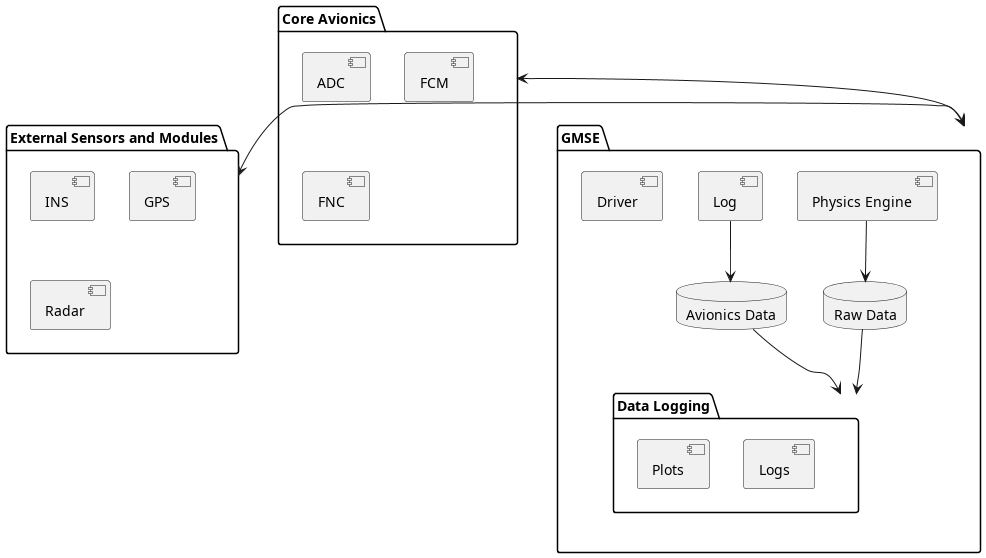
\includegraphics[width=\textwidth]{high-level}
\caption{}
\label{fig:high-level}
\end{figure*}
